%Copyright 2014 Jean-Philippe Eisenbarth
%This program is free software: you can 
%redistribute it and/or modify it under the terms of the GNU General Public 
%License as published by the Free Software Foundation, either version 3 of the 
%License, or (at your option) any later version.
%This program is distributed in the hope that it will be useful,but WITHOUT ANY 
%WARRANTY; without even the implied warranty of MERCHANTABILITY or F2ITNESS FOR A 
%PARTICULAR PURPOSE. See the GNU General Public License for more details.
%You should have received a copy of the GNU General Public License along with 
%this program.  If not, see <http://www.gnu.org/licenses/>.

%Based on the code of Yiannis Lazarides
%http://tex.stackexchange.com/questions/42602/software-requirements-specification-with-latex
%http://tex.stackexchange.com/users/963/yiannis-lazarides
%Also based on the template of Karl E. Wiegers
%http://www.se.rit.edu/~emad/teaching/slides/srs_template_sep14.pdf
%http://karlwiegers.com
\documentclass{report}
\usepackage{listings}
\usepackage{underscore}
\usepackage[bookmarks=true]{hyperref}
\usepackage[utf8]{inputenc}
\usepackage{multirow}
\usepackage[table,xcdraw]{xcolor}
\usepackage[english]{babel}
\usepackage{graphicx}
\usepackage{caption}
\usepackage{subcaption}
\usepackage{wrapfig}
\usepackage[toc,xindy]{glossaries}
\usepackage{verbatim}
\usepackage{hyperref}
\usepackage[toc]{appendix}
\usepackage{booktabs}
\usepackage{amsmath}
\usepackage{grffile}
\newcommand{\addcustomplot}[4]{	
	{
		%\pgfplotstablegetcolsof{#}
		\addplot[scatter, color=#2,
		scatter/@pre marker code/.style={/tikz/mark size=2.0pt},
		scatter/@post marker code/.style={},
		line width = 1.5pt
		]
		table[x index=0,y index=#3, col sep=comma] {#1};
		\addlegendentryexpanded{#4}
	}
}

\newcommand{\addcustomybarplot}[4]
{
	\addplot[black,pattern color=#3,fill=#3,pattern=north east lines]  table[x index=0,y index=#2,col sep=comma]{#1};
	\addlegendentryexpanded{#4};
}


\newcommand{\plotfile}[1]{
	\pgfplotstableread{#1}{\table}
	\pgfplotstablegetcolsof{#1}
	\pgfmathtruncatemacro\numberofcols{\pgfplotsretval-1}
	\pgfplotsinvokeforeach{1,...,\numberofcols}{
		\pgfplotstablegetcolumnnamebyindex{##1}\of{\table}\to{\colname}
		\addplot table [y index=##1] {#1}; 
		\addlegendentryexpanded{\colname}
	}
}

\newcommand{\stencilpt}[4][]{\node[circle,draw,inner sep=0.1em,minimum size=0.8cm,font=\tiny,#1] at (#2) (#3) {#4}}


\lstset{
	basicstyle=\ttfamily\footnotesize,
	frame=single,
	breaklines=true,
	postbreak=\raisebox{0ex}[0ex][0ex]{\ensuremath{\color{red}\hookrightarrow\space}}
}


% Define block styles
\tikzstyle{decision} = [diamond, draw, fill=blue!20, 
text width=4.5em, text badly centered, node distance=3cm, inner sep=0pt]
\tikzstyle{block} = [rectangle, draw, fill=blue!20, 
 text centered, rounded corners, minimum height=4em, node distance=3cm]
\tikzstyle{line} = [draw, -latex']
\tikzstyle{cloud} = [draw, ellipse,fill=red!20, node distance=3cm,
minimum height=2em]
\usepackage{listings}
\usepackage{underscore}
\usepackage{grffile}
\setcounter{secnumdepth}{5}
\usepackage[bookmarks=true]{hyperref}
\usepackage[utf8]{inputenc}
\usepackage[english]{babel}
\hypersetup{
    bookmarks=false,    % show bookmarks bar?
    pdftitle={Software Requirement Specification},    % title
    pdfauthor={Mateusz Gasior},                     % author
    pdfsubject={TeX and LaTeX},                        % subject of the document
    pdfkeywords={TeX, LaTeX, graphics, images}, % list of keywords
    colorlinks=true,       % false: boxed links; true: colored links
    linkcolor=blue,       % color of internal links
    citecolor=black,       % color of links to bibliography
    filecolor=black,        % color of file links
    urlcolor=purple,        % color of external links
    linktoc=page            % only page is linked
}%
\def\myversion{1.0 }
\date{}
%\title
\usepackage{hyperref}
\begin{document}

\begin{flushright}
    \rule{16cm}{5pt}\vskip1cm
    \begin{bfseries}
        \Huge{SOFTWARE REQUIREMENTS\\ SPECIFICATION}\\
        \vspace{1.9cm}
        for\\
        \vspace{1.9cm}
        Requirements Analysis and System Design 
        \& 
        Software Testing and Quality Assurance \\
        \vspace{1.9cm}
        \LARGE{Version \myversion approved}\\
        \vspace{1.9cm}
        Prepared by Mateusz Gasior\\
        \vspace{1.9cm}
        Cranfield University\\
        \vspace{1.9cm}
        \today\\
    \end{bfseries}
\end{flushright}

\tableofcontents


\chapter*{Revision History}

\begin{center}
    \begin{tabular}{|c|c|c|c|}
        \hline
	    Name & Date & Reason For Changes & Version\\
        \hline
	    21 & 22 & 23 & 24\\
        \hline
	    31 & 32 & 33 & 34\\
        \hline
    \end{tabular}
\end{center}

\chapter{Introduction}

\section{Purpose}
%$<$Identify the product whose software requirements are specified in this 
%document, including the revision or release number. Describe the scope of the 
%product that is covered by this SRS, particularly if this SRS describes only 
%part of the system or a single subsystem.$>$
For purposes of assignment University is in the process of acquiring a new supercomputer to support
research activities. This task requires a proper hardware, safe accessibility of the user and smart scheduler
for managing submitted jobs. In terms of this process university requires a simulation tool to model the behavior of the computing platform and to establish good accounting practices. 

In chapter \ref{chp:sc} are requirements connected to supercomputer and computing platform itself, which may be useful to understand the idea and possibility of the system, although there would not be used in modeling of simulation tool. Next chapter \ref{chp:sim} contains all extracted requirements for simulation tool.

\section{Document Conventions}
%$<$Describe any standards or typographical conventions that were followed when 
%writing this SRS, such as fonts or highlighting that have special significance.  
%For example, state whether priorities  for higher-level requirements are assumed 
%to be inherited by detailed requirements, or whether every requirement statement 
%is to have its own priority.$>$
Every requirement has a unique name/code which for identification. The prefix of single feature's identification code remains the same, only the suffix changes by an auto-increment integer value. In some cases also additional mid-term can occur between prefix and suffix to precisely describe requirement. Additionally for each feature there can be constructed a glossary, which is mentioned in the correct section and placed in an appendix. 
\section{Intended Audience and Reading Suggestions}
%$<$Describe the different types of reader that the document is intended for, 
%such as developers, project managers, marketing staff, users, testers, and 
%documentation writers. Describe what the rest of this SRS contains and how it is 
%organized. Suggest a sequence for reading the document, beginning with the 
%overview sections and proceeding through the sections that are most pertinent to 
%each reader type.$>$
The core of software requirements specification document is stored in chapter \ref{chp:sim}, although in chapter \ref{chp:sc} contains additional information which can be used to better describe properties of developed software. The suggestion is to start reading documentation as it is, with order of the table of content. Each of the chapters and sections can contain additional diagrams placed in appendix. 

\section{Project Scope}
%$<$Provide a short description of the software being specified and its purpose, 
%including relevant benefits, objectives, and goals. Relate the software to 
%corporate goals or business strategies. If a separate vision and scope document 
%is available, refer to it rather than duplicating its contents here.$>$

The purpose of the project is to design and develop simulation tool for supercomputer platform. The goal is to have a tool which by changing different parameters can model different accounting practices of such platform. The benefit is clearly visible, first of all the university could be able to model different accounting practices for different load of jobs/tasks in a system. This kind of approach doesn't have big advantage comparing to real-time introducing changes in accounting practices -- it can be tested in controlled environment.
 
%\section{References}
%$<$List any other documents or Web addresses to which this SRS refers. These may 
%include user interface style guides, contracts, standards, system requirements 
%specifications, use case documents, or a vision and scope document. Provide 
%enough information so that the reader could access a copy of each reference, 
%including title, author, version number, date, and source or location.$>$


\chapter{Overall Description}

\section{Product Perspective}
%$<$Describe the context and origin of the product being specified in this SRS.  
%For example, state whether this product is a follow-on member of a product 
%family, a replacement for certain existing systems, or a new, self-contained 
%product. If the SRS defines a component of a larger system, relate the 
%requirements of the larger system to the functionality of this software and 
%identify interfaces between the two. A simple diagram that shows the major 
%components of the overall system, subsystem interconnections, and external 
%interfaces can be helpful.$>$

The idea of simulation tool started with the process of acquiring a new supercomputer in order to support research activities by university. The need of a new product was established by replacing the existing system to a newer one.

\section{Product Functions}
%$<$Summarize the major functions the product must perform or must let the user 
%perform. Details will be provided in Section 3, so only a high level summary 
%(such as a bullet list) is needed here. Organize the functions to make them 
%understandable to any reader of the SRS. A picture of the major groups of 
%related requirements and how they relate, such as a top level data flow diagram 
%or object class diagram, is often effective.$>$

The main function of simulation tool is to model behavior of computation platform. Each simulation can have different input parameters and should produce according to the parametrization correct output.

%\section{User Classes and Characteristics}
%$<$Identify the various user classes that you anticipate will use this product.  
%User classes may be differentiated based on frequency of use, subset of product 
%functions used, technical expertise, security or privilege levels, educational 
%level, or experience. Describe the pertinent characteristics of each user class.  
%Certain requirements may pertain only to certain user classes. Distinguish the 
%most important user classes for this product from those who are less important 
%to satisfy.$>$

\section{Operating Environment}
%$<$Describe the environment in which the software will operate, including the 
%hardware platform, operating system and versions, and any other software 
%components or applications with which it must peacefully coexist.$>$

The project is a basic simulation tool which is able to model all the behavior in a virtual way. From that reason it is possible to ensure a platform independent solution.

\section{Design and Implementation Constraints}
%$<$Describe any items or issues that will limit the options available to the 
%developers. These might include: corporate or regulatory policies; hardware 
%limitations (timing requirements, memory requirements); interfaces to other 
%applications; specific technologies, tools, and databases to be used; parallel 
%operations; language requirements; communications protocols; security 
%considerations; design conventions or programming standards (for example, if the 
%customer’s organization will be responsible for maintaining the delivered 
%software).$>$

At the point of design and implementation there are no limits of issues connected with the technology restrictions or policy issues.

\section{User Documentation}
%$<$List the user documentation components (such as user manuals, on-line help, 
%and tutorials) that will be delivered along with the software. Identify any 
%known user documentation delivery formats or standards.$>$

The user manual with the source code is in other document named \textbf{UserGuideAndSourceFiles.pdf}. This document contains basic example of usage of simulation tool, diagrams related to the structure of program.

%\section{Assumptions and Dependencies}

%$<$List any assumed factors (as opposed to known facts) that could affect the 
%requirements stated in the SRS. These could include third-party or commercial 
%components that you plan to use, issues around the development or operating 
%environment, or constraints. The project could be affected if these assumptions 
%are incorrect, are not shared, or change. Also identify any dependencies the 
%project has on external factors, such as software components that you intend to 
%reuse from another project, unless they are already documented elsewhere (for 
%example, in the vision and scope document or the project plan).$>$


%\chapter{External Interface Requirements}

%\section{User Interfaces}
%$<$Describe the logical characteristics of each interface between the software 
%product and the users. This may include sample screen images, any GUI standards 
%or product family style guides that are to be followed, screen layout 
%constraints, standard buttons and functions (e.g., help) that will appear on 
%every screen, keyboard shortcuts, error message display standards, and so on.  
%Define the software components for which a user interface is needed. Details of 
%the user interface design should be documented in a separate user interface 
%specification.$>$

%\section{Hardware Interfaces}
%$<$Describe the logical and physical characteristics of each interface between 
%the software product and the hardware components of the system. This may include 
%the supported device types, the nature of the data and control interactions 
%between the software and the hardware, and communication protocols to be 
%used.$>$

%\section{Software Interfaces}
%$<$Describe the connections between this product and other specific software 
%components (name and version), including databases, operating systems, tools, 
%libraries, and integrated commercial components. Identify the data items or 
%messages coming into the system and going out and describe the purpose of each.  
%Describe the services needed and the nature of communications. Refer to 
%documents that describe detailed application programming interface protocols.  
%Identify data that will be shared across software components. If the data 
%sharing mechanism must be implemented in a specific way (for example, use of a 
%global data area in a multitasking operating system), specify this as an 
%implementation constraint.$>$

%\section{Communications Interfaces}
%$<$Describe the requirements associated with any communications functions 
%required by this product, including e-mail, web browser, network server 
%communications protocols, electronic forms, and so on. Define any pertinent 
%message formatting. Identify any communication standards that will be used, such 
%as FTP or HTTP. Specify any communication security or encryption issues, data 
%transfer rates, and synchronization mechanisms.$>$

%\chapter{System Features}
$<$This template illustrates organizing the functional requirements for the 
product by system features, the major services provided by the product. You may 
prefer to organize this section by use case, mode of operation, user class, 
object class, functional hierarchy, or combinations of these, whatever makes the 
most logical sense for your product.$>$
\chapter{Hardware requirements} \label{sec:hardware_requirements}
	Mentioned in this chapter requirements are for job controller which should be able to handle with hardware in the most optimal way.
	
	\section{Demands of customer}
	\label{sec:hardware_requirements_demands}
		The system is heterogeneous system containing:
		\begin{itemize}
			\item A set of "traditional" computing nodes, i.e. shared-memory multi-core CPUs;
			\item A set of "accelerated" computing node, same as above  but with 1 or 2 attached GPUs dedicated to computations;
			\item A set of specialized nodes, with GPUs dedicated to rendering and visualization of complex data;
			\item A set of storage devices.
		\end{itemize}
		The system should manage at least $128$ nodes with at least $16$ processor cores per node.
	
	\section{Glossary} 
	\label{sec:hardware_requirements_glossary}
		The glossary for hardware requirements in this chapter is presented in Table \ref{tab:hardware_requirements_glossary}. Information stored in this table refers to section \ref{sec:hardware_requirements_demands}. Each key found in the mentioned section is described and will be used in other section in order to be consistent with terminology.
		\begin{table}[!htbp]
			\centering
			\caption{Glossary for hardware requirements.}
			\label{tab:hardware_requirements_glossary}
			\begin{tabular}{|c|c|}
				\hline
				\textbf{Key} & \textbf{Description} \\ \hline \hline
				Node & It's shared-memory multi-core CPU.\\ \hline
				Computing node & It's a node used for computation. \\ \hline
				\multirow{2}{*}{Accelerated node} &  It's a computing node with attached 1 or 2 \\ & GPUs dedicated to computations.\\ \hline
				\multirow{2}{*}{Specialized node} & It's a traditional computing node with GPU \\& dedicated to rendering and visualization of complex data. \\ \hline \hline
				Storage device & It's device that can store information, generally hard-drives. \\ \hline
			\end{tabular}
		\end{table}
	
	\section{List of requirements}
		Based on the demands of customer in section \ref{sec:hardware_requirements_demands} and glossary in section \ref{sec:hardware_requirements_glossary} list of requirements was created. It is presented in Table \ref{tab:hardware_requirements_list}. 
	
		\begin{table}[!htbp]
			\centering
			\caption{Hardware requirements list.}
			\label{tab:hardware_requirements_list}
			\begin{tabular}[width=\textwidth]{|c|c|l|}
				\hline
				\textbf{Ref no.} & \textbf{Name} & \multicolumn{1}{c|}{\textbf{Description}} \\ \hline \hline
				HRD\_1 & \textit{\textbf{Managing different types of nodes.}} & \begin{tabular}[c]{@{}l@{}}The system should manage different types of nodes:\\ traditional, accelerated and specialized.\end{tabular} \\ \hline
				HRD\_2 & \textit{\textbf{Managing traditional nodes.}} & The system should manage traditional nodes. \\ \hline
				HRD\_3 & \textit{\textbf{Managing of accelerated nodes.}} & The system should manage accelerated nodes. \\ \hline
				HRD\_4 & \textit{\textbf{Managing specialized nodes.}} & The system should manage specialied nodes. \\ \hline
				HRD\_5 & \textit{\textbf{Managing storage devices.}} & The system should manage multiple storage devices. \\ \hline
				HRD\_6 & \textit{\textbf{Managing at least 128 nodes.}} & \begin{tabular}[c]{@{}l@{}}The system should manage at least\\ 128 different nodes.\end{tabular} \\ \hline
				HRD\_7 & \textit{\textbf{\begin{tabular}[c]{@{}c@{}}Managing nodes with at least \\ 16 processors cores.\end{tabular}}} & \begin{tabular}[c]{@{}l@{}}The system should manage nodes with \\ at least 16 processor cores.\end{tabular} \\ \hline
			\end{tabular}
		\end{table}
\chapter{User requirements} \label{sec:user_requirements}
	Mentioned in this chapter requirements are related to users in a system. User can have many users, which should be able to work simultaneously. Users are in groups and have different sizes.
	
	\section{Demands of customer}
	\label{sec:user_requirements_demands}
		The users of the system can be classified as:
		\begin{itemize}
			\item IT support;
			\item Researchers;
			\item Students;
		\end{itemize}
		Researchers are divided into groups, according to the department structure, where each group has an allocation of resources, but individual researchers may have grants entitling them to additional resource usage.
		
		Students are grouped by the curriculum they are enrolled in, and all students have a cap on the maximum usable resources, both cumulative and instantaneous, which may depend on their group.
	
	\section{Glossary} 
	\label{sec:user_requirements_glossary}
		The glossary for user requirements in this chapter is presented in Table \ref{tab:user_requirements_glossary}. Information stored in this table refers to section \ref{sec:user_requirements_demands}. Each key found in the mentioned section is described and will be used in other section in order to be consistent with terminology.
		\begin{table}[!htbp]
			\centering
			\caption{Glossary for user requirements.}
			\label{tab:user_requirements_glossary}
			\begin{tabular}{|l|l|}
				\hline
				\textbf{Key} & \textbf{Description} \\ \hline \hline
				It support member & Actor in the system. \\ \hline
				Researcher & Actor in the system. \\ \hline
				Student & Actor in the system. \\ \hline
				Resources & Resources to be understood as an access to:\\& nodes; cores; storage and machine time.\\ \hline
				Grant & Entitles actor of a system to additional resource usage. \\ \hline
			\end{tabular}
		\end{table}
	
	\section{List of requirements}
		Based on the demands of customer in section \ref{sec:user_requirements_demands} and glossary in section \ref{sec:user_requirements_glossary} list of requirements was created. It is presented in Table \ref{tab:user_requirements_list}. 
	
		\begin{table}[!htbp]
			\centering
			\caption{User requirements list.}
			\label{tab:user_requirements_list}
			\begin{tabular}[width=\textwidth]{|c|c|l|}
				\hline
				\textbf{Ref no.} & \textbf{Name} & \multicolumn{1}{c|}{\textbf{Description}} \\ \hline \hline
				USR\_1 & \textit{\textbf{Researchers are divided into groups.}} & \begin{tabular}[c]{@{}l@{}}Each researcher is grouped according to \\department structure. Should be in a group.\end{tabular} \\ \hline
				USR\_2 & \textit{\textbf{Researcher group has a limit of resources.}} & \begin{tabular}[c]{@{}l@{}}Each group has different permissions connected \\ with available resources in a system.\end{tabular} \\ \hline
				USR\_3 & \textit{\textbf{Researcher can have additional permissions.}} & \begin{tabular}[c]{@{}l@{}}Particular researcher can have grant, which\\ gives more resources to usage.\end{tabular} \\ \hline \hline
				USR\_4 & \textit{\textbf{Students are grouped by enrolled programs.}} & \begin{tabular}[c]{@{}l@{}}Each student has to be in a group, corresponded \\ to the program.\end{tabular} \\ \hline
				USR\_5 & \textit{\textbf{Student have a cap on resources.}} & \begin{tabular}[c]{@{}l@{}}Each student have a cap on maximum usable \\ resources. Both cumulative and instantaneous, \\ which may depend on their group.\end{tabular} \\ \hline
				USR\_6 & \textit{\textbf{Student groups have limits for single use.}} & \begin{tabular}[c]{@{}l@{}}Instantaneous cap are correlated with student \\ groups.\end{tabular} \\ \hline
				USR\_7 & \textit{\textbf{Student groups have limits per usages.}} & \begin{tabular}[c]{@{}l@{}}Cumulative cap are correlated with student \\ groups.\end{tabular} \\ \hline
			\end{tabular}
		\end{table}
	
		Allocation of resources for research groups should be understood as continuous access to some amount of processors and storage in the system. Resources are shared between group, which means that if one of the researchers uses all research, no one of the rest can use it in the same time. A difference between student and research group is that for first one has allocation of resources and the second one has restrictions, caps and limits. The common parts are instantaneous limits, i.e. limit of processors per usage.
\chapter{Scheduler requirements} \label{sec:scheduler_requirements}
	Mentioned in this chapter requirements are related to scheduling in a system. Users can submit many jobs in a different queues. The role of a scheduling system is to optimally use resources, which can be understood as minimizing waiting time or maximize utilization. 
	
	\section{Demands of customer}
	\label{sec:scheduler_requirements_demands}
		The system shall match job requests to resources; there will be different classes of jobs for different uses, e.g. short, medium, long running, interactive, etc. The job requests should be serviced in an order established by an auxiliary algorithm called a scheduler; for the purposes of this exercise, a first-come first-served approach is acceptable, even though in a real computing center more sophisticated algorithms would need to be employed. In particular, the system should be used "optimally" in a sense to be clarified, bearing in mind that different stakeholders may have different optimality criteria; for instance, users want to minimize waiting time, whereas system administrator have to maximize utilization. The university IT department needs a simulation tool to model the behavior of the computing platform and to establish good accounting practices. The policy constraints are:
		\begin{itemize}
			\item
			{
				 There are at least four different job queues:
				 \begin{enumerate}
				 	\item Short, interactive jobs that can take up to $2$ nodes for no more than 1 hour; a certain subset (say $10\%$) of the machine must be reserved for this queue;
				 	\item Medium-sized jobs that can take up to $10\%$ of the total number of cores, and can last up to $8$ hours; another subset (say $30\%$) of the machine must be reserved for this queue;
				 	\item Large jobs, that can take up to $16$ hours and up to $50\%$ of the total core count;
				 	\item Huge, active only from $0500pm$ Friday to $0900am$ Monday, where the jobs can potentially reserve the whole machine. During there times the other job queues do not serve requests.
				 \end{enumerate}
			}
			\item Each job queue has associated a cost for number of machine-hours requested.
			\item Each job will request a certain number of processor cores for a certain amount of time. For the sake of simplicity you can assume that, at any given time, the queuing software will grant access under a first-come first-served basis, up to available capacity of the machine.
			\item At the end of the week, there will be a cutoff time such that no new jobs will start if their estimated completion time will go beyond the end of the work week (thereby leaving the machine free for the weekend queue).
		\end{itemize}
		
		
	\section{Glossary} 
	\label{sec:scheduler_requirements_glossary}
		The glossary for user requirements in this chapter is presented in Table \ref{tab:scheduler_requirements_glossary}. Information stored in this table refers to section \ref{sec:scheduler_requirements_demands}. Each key found in the mentioned section is described and will be used in other section in order to be consistent with terminology.
		\begin{table}[!htbp]
			\centering
			\caption{Glossary for scheduler requirements.}
			\label{tab:scheduler_requirements_glossary}
			\begin{tabular}{|l|l|}
				\hline
				\textbf{Key} & \textbf{Description} \\ \hline \hline
				Job & A task submitted by a user to a system. \\ \hline
				Reserved resources & Resources reserved for a specific queuing in the system.\\ \hline
				Cutoff time & \begin{tabular}[c]{@{}l@{}}Time which doesn't allow a new jobs to execute if their \\ execution time would exceed start of a weekend.\end{tabular}\\ \hline
			\end{tabular}
		\end{table}
	
	\section{List of requirements}
		Based on the demands of customer in section \ref{sec:scheduler_requirements_demands} and glossary in section \ref{sec:scheduler_requirements_glossary} list of requirements was created. It is presented in Table \ref{tab:scheduler_requirements_list}. Requirements from this chapter are partially formed for simulator needs. There are many assumptions in demands of customer -- University. Some of the demands are super precise, which makes the system less flexible for changes.
	
		\begin{table}[!htbp]
			\centering
			\caption{Scheduler requirements list.}
			\label{tab:scheduler_requirements_list}
			\begin{tabular}[width=\textwidth]{|c|c|l|}
				\hline
				\textbf{Ref no.} & \textbf{Name} & \multicolumn{1}{c|}{\textbf{Description}} \\ \hline \hline
				SCR\_1 & \textit{\textbf{Scheduler serving approach.}} & \begin{tabular}[c]{@{}l@{}}Scheduler can use firs-come first-served approach.\end{tabular} \\ \hline
				SCR\_2 & \textit{\textbf{The system should be used optimally.}} & \begin{tabular}[c]{@{}l@{}}System should minimize or maximize some criteria \\ in order to be optimal.\end{tabular} \\ \hline
				SCR\_3 & \textit{\textbf{Four job queues.}} & \begin{tabular}[c]{@{}l@{}}There are four different job queues.\end{tabular} \\ \hline \hline
				SCR\_4 & \textit{\textbf{Short job queue.}} & \begin{tabular}[c]{@{}l@{}}There is an interactive short job queue.\end{tabular} \\ \hline
				SCR\_4\_A & \textit{\textbf{Short job queue restrictions.}} & \begin{tabular}[c]{@{}l@{}}Job can take up to 2 nodes for no more than 1 hour.\end{tabular} \\ \hline
				SCR\_4\_B & \textit{\textbf{Short job queue reservations.}} & \begin{tabular}[c]{@{}l@{}}Subset of $10\%$ should be reserved for this queue. \end{tabular} \\ \hline \hline
				SCR\_5 & \textit{\textbf{Medium-sized (MS) job queue.}} & \begin{tabular}[c]{@{}l@{}}There is a medium-sized job queue.\end{tabular} \\ \hline
				SCR\_6\_A & \textit{\textbf{MS job queue restrictions.}} & \begin{tabular}[c]{@{}l@{}} Job can take up to $10\%$ of the total number of cores \\ for no more than 8 hours.\end{tabular} \\ \hline
				SCR\_6\_B & \textit{\textbf{MS job queue reservations.}} & \begin{tabular}[c]{@{}l@{}}Subset of $30\%$ of the machine should be reserved \\ for this queue.\end{tabular} \\ \hline \hline
				SCR\_7 & \textit{\textbf{Large job queue.}} & \begin{tabular}[c]{@{}l@{}}There is a large job queue in a system.\end{tabular} \\ \hline
				SCR\_7\_A & \textit{\textbf{Large job queue restrictions.}} & \begin{tabular}[c]{@{}l@{}}Job can take up to 6 hours and consume $50\%$ of \\ total core count.\end{tabular} \\ \hline \hline
				SCR\_8 & \textit{\textbf{Huge job queue.}} & \begin{tabular}[c]{@{}l@{}}There is a huge job queue in the system.\end{tabular} \\ \hline
				SCR\_8\_A & \textit{\textbf{Huge job queue restrictions.}} & \begin{tabular}[c]{@{}l@{}}This queue works from $0500pm$ Friday to $0900am$ \\ Monday, where the jobs can potentially reserve \\ the whole machine.\end{tabular} \\ \hline
				SCR\_8\_B & \textit{\textbf{Huge job queue uniqueness.}} & \begin{tabular}[c]{@{}l@{}}During working time of this queue other queues \\ don't work.\end{tabular} \\ \hline \hline
				SCR\_9 & \textit{\textbf{Associated cost.}} & \begin{tabular}[c]{@{}l@{}}Each of queue in the system has associated cost \\ based on requested machine-hours.\end{tabular} \\ \hline
				SCR\_10 & \textit{\textbf{Requesting number of processors core.}} & \begin{tabular}[c]{@{}l@{}}At any given time, the queuing software will grant \\ access under a FCFS basis, up to available capacity \\ of the machine.\end{tabular} \\ \hline
				SCR\_11 & \textit{\textbf{Cutoff time.}} & \begin{tabular}[c]{@{}l@{}}No new jobs will start if their estimated completion \\ time will go beyond the end of the work week \\ (SCR\_8\_A).\end{tabular} \\ \hline
			\end{tabular}
		\end{table}
	
\section{System Feature 1}
$<$Don’t really say “System Feature 1.” State the feature name in just a few 
words.$>$

\subsection{Description and Priority}
$<$Provide a short description of the feature and indicate whether it is of 
High, Medium, or Low priority. You could also include specific priority 
component ratings, such as benefit, penalty, cost, and risk (each rated on a 
relative scale from a low of 1 to a high of 9).$>$

\subsection{Stimulus/Response Sequences}
$<$List the sequences of user actions and system responses that stimulate the 
behavior defined for this feature. These will correspond to the dialog elements 
associated with use cases.$>$

\subsection{Functional Requirements}
$<$Itemize the detailed functional requirements associated with this feature.  
These are the software capabilities that must be present in order for the user 
to carry out the services provided by the feature, or to execute the use case.  
Include how the product should respond to anticipated error conditions or 
invalid inputs. Requirements should be concise, complete, unambiguous, 
verifiable, and necessary. Use “TBD” as a placeholder to indicate when necessary 
information is not yet available.$>$

$<$Each requirement should be uniquely identified with a sequence number or a 
meaningful tag of some kind.$>$

REQ-1:	REQ-2:

\section{System Feature 2 (and so on)}


\chapter{Other Nonfunctional Requirements}

\section{Performance Requirements}
$<$If there are performance requirements for the product under various 
circumstances, state them here and explain their rationale, to help the 
developers understand the intent and make suitable design choices. Specify the 
timing relationships for real time systems. Make such requirements as specific 
as possible. You may need to state performance requirements for individual 
functional requirements or features.$>$

\section{Safety Requirements}
$<$Specify those requirements that are concerned with possible loss, damage, or 
harm that could result from the use of the product. Define any safeguards or 
actions that must be taken, as well as actions that must be prevented. Refer to 
any external policies or regulations that state safety issues that affect the 
product’s design or use. Define any safety certifications that must be 
satisfied.$>$

\section{Security Requirements}
$<$Specify any requirements regarding security or privacy issues surrounding use 
of the product or protection of the data used or created by the product. Define 
any user identity authentication requirements. Refer to any external policies or 
regulations containing security issues that affect the product. Define any 
security or privacy certifications that must be satisfied.$>$

\section{Software Quality Attributes}
$<$Specify any additional quality characteristics for the product that will be 
important to either the customers or the developers. Some to consider are: 
adaptability, availability, correctness, flexibility, interoperability, 
maintainability, portability, reliability, reusability, robustness, testability, 
and usability. Write these to be specific, quantitative, and verifiable when 
possible. At the least, clarify the relative preferences for various attributes, 
such as ease of use over ease of learning.$>$

\section{Business Rules}
$<$List any operating principles about the product, such as which individuals or 
roles can perform which functions under specific circumstances. These are not 
functional requirements in themselves, but they may imply certain functional 
requirements to enforce the rules.$>$


\chapter{System Features}
$<$This template illustrates organizing the functional requirements for the 
product by system features, the major services provided by the product. You may 
prefer to organize this section by use case, mode of operation, user class, 
object class, functional hierarchy, or combinations of these, whatever makes the 
most logical sense for your product.$>$

\chapter{Supercomputer features} \label{chp:sc}
% HARDWARE FEATURES
\section{Hardware features}

\subsection{Description and Priority}
%{Provide a short description of the feature and indicate whether it is of 
%High, Medium, or Low priority. You could also include specific priority 
%component ratings, such as benefit, penalty, cost, and risk (each rated on a 
%relative scale from a low of 1 to a high of 9).

Mentioned in this chapter features are related to the lowest layer of supercomputer, which in short describes of what components should be managed by a system. Features of this type have a really high priority, because they determine the supercomputer as a whole. Mentioned requirements stands for a hearth of a supercomputer and system. Glossary for this feature is in appendix \ref{app:glossary:hardware}.

%\subsection{Stimulus/Response Sequences}
%$<$List the sequences of user actions and system responses that stimulate the 
%behavior defined for this feature. These will correspond to the dialog elements 
%associated with use cases.$>$

\subsection{Functional Requirements}
%$<$Itemize the detailed functional requirements associated with this feature.  
%These are the software capabilities that must be present in order for the user 
%to carry out the services provided by the feature, or to execute the use case.  
%Include how the product should respond to anticipated error conditions or 
%invalid inputs. Requirements should be concise, complete, unambiguous, 
%verifiable, and necessary. Use “TBD” as a placeholder to indicate when necessary 
%information is not yet available.$>$

%$<$Each requirement should be uniquely identified with a sequence number or a 
%meaningful tag of some kind.$>$
Subsections below are a list of a requirements related to the hardware feature.
Requirements extracted from user demands:
\begin{itemize}
	\item
	{
		\textbf{HRD-1} -- The system should manage different types of nodes: traditional, accelerated and specialized.	
	}
	\item
	{
		\textbf{HRD-2} -- The system should manage traditional nodes.
	}
	\item
	{
		\textbf{HRD-3} -- The system should manage accelerated nodes.
	}
	\item
	{
		\textbf{HRD-4} -- The system should manage specialized nodes.
	}
	\item
	{
		\textbf{HRD-5} -- The system should manage multiple storage devices.
	}
	\item
	{
		\textbf{HRD-6} -- The system should manage at least $128$ different nodes.
	}
	\item
	{
		\textbf{HRD-7} -- The system should manage nodes with at least $16$ processor cores.
	}
\end{itemize}

% END OF HARDWARE FEATURES

% USER FEATURES
\section{User features} \label{sec:uf}

\subsection{Description and Priority}
%{Provide a short description of the feature and indicate whether it is of 
%High, Medium, or Low priority. You could also include specific priority 
%component ratings, such as benefit, penalty, cost, and risk (each rated on a 
%relative scale from a low of 1 to a high of 9).
Mentioned in this chapter requirements are related to the users in a supercomputer system. System distinguish some type of users, which are differently accounted. Each of users can have different permissions. Users can be connected and gathered in a groups, which can have a permissions. 
Glossary for this feature is in appendix \ref{app:glossary:user}.

\subsection{Stimulus/Response Sequences}
%$<$List the sequences of user actions and system responses that stimulate the 
%behavior defined for this feature. These will correspond to the dialog elements 
%associated with use cases.$>$
Requirements in this chapter are related to the structure of users using supercomputer. Some of requirements were extracted from the customer demands, but the other part had to be found during requirement analysis.
\subsection{Functional Requirements}
%$<$Itemize the detailed functional requirements associated with this feature.  
%These are the software capabilities that must be present in order for the user 
%to carry out the services provided by the feature, or to execute the use case.  
%Include how the product should respond to anticipated error conditions or 
%invalid inputs. Requirements should be concise, complete, unambiguous, 
%verifiable, and necessary. Use “TBD” as a placeholder to indicate when necessary 
%information is not yet available.$>$

%$<$Each requirement should be uniquely identified with a sequence number or a 
%meaningful tag of some kind.$>$
Subsections below are a list of a requirements related to the user feature.
Requirements extracted from user demands:
\begin{itemize}
	\item
	{
		\textbf{USR-1} -- Each researcher is grouped according to department structure. Should be in a group.
	}
	\item
	{
		\textbf{USR-2} -- Each researcher group has different permissions connected with available resources in a system (Has a limit on resources).
	}
	\item
	{
		\textbf{USR-3} -- particular researcher can have a grant, which gives more resources to usage (Gives additional permissions).
	}
	\item
	{
		\textbf{USR-4} -- Students are grouped by enrolled programs. Student has to be in a group.
	}
	\item
	{
		\textbf{USR-5} -- Each student has a cp on maximum usable resources. Both cumulative and instantaneous, which may depend on their group. Look at requirements \textbf{USR-6} and \textbf{USR-7}.
	}
	\item
	{
		\textbf{USR-6} -- Instantaneous cap is correlated with student groups. It describes how many processors, nodes student can use at once (single use).
	}
	\item
	{
		\textbf{USR-7} -- Cumulative cap is correlated with a student group. It gives an information about cumulative usage of a supercomputer in range of dates, for example student can only use machine for $8h$ monthly.
	}
	\item
	{
		\textbf{USR-8} -- Students and researchers can submit tasks/jobs to the system according to their privileges and restrictions.
	}
\end{itemize}

	Allocation of resource for research groups should be understood as continuous access to some amount of processors and storage in the system. Resources are shared between group, which means that if one of the researchers uses all resources, no on of the rest can use it in the same time. A difference between student and research group is that: firstly allocation of resources and secondly restrictions, caps and limits. The common parts are instantaneous limits, i.e. limits of processors per usage.
	
Requirement extracted during analysis:
\begin{itemize}
	\item
	{
		\textbf{USR-A-1} -- Only IT supporter should be able to manage structure of users in a system.
	}
	\item
	{
		\textbf{USR-A-2} -- IT supporter should be able to create a research group.
	}
	\item
	{
		\textbf{USR-A-3} -- IT supporter should be able to modify a research group.
	}
	\item
	{
		\textbf{USR-A-4} -- IT supporter should be able to delete a research group.
	}
	\item
	{
		\textbf{USR-A-5} -- It supporter should be able to add permissions to a research group.
	}
	\item
	{
		\textbf{USR-A-6} -- IT supporter should be able to add allocation of resources to a research group.
	}
	\item
	{
		\textbf{USR-A-7} -- IT supporter should be able to add users to a research group.
	}
	\item
	{
		\textbf{USR-A-8} -- IT supporter should be able to add user to a system.
	}
	\item
	{
		\textbf{USR-A-9} -- IT supporter should be able to modify user permissions (grants).
	}
	\item
	{
		\textbf{USR-A-10} -- IT supporter should be able to create student group.
	}
	\item
	{
		\textbf{USR-A-11} -- IT supporter should be able to add permissions to a student group.
	}
	\item
	{
		\textbf{USR-A-12} -- IT supporter should be able to add restrictions (caps) to a student group.
	}
	\item
	{
		\textbf{USR-A-13} -- IT supporter should be able to add members to a student group.
	}
	\item
	{
		\textbf{USR-A-14} -- IT supporter should be able to remove members from a student group.
	}
	\item
	{
		\textbf{USR-A-15} -- IT supporter should be able to remove members from a research group.
	}
\end{itemize}
	During the analysis found a incoherence about the amount of resources in the system connected to the single user. In consequences assumption were made as follows: if user is in a multiple groups (in terms of research of student groups) his account balance is added, in other words user would be able to use all permissions and all balances from all groups that he belongs into. Restrictions to the users are based on the student group only so, if user belongs to multiple groups the restriction is applied only in terms of a group that he use for submitting the job to the system.
% END OF USER FEATURES

% JOB CONTROLLER FEATURES

\section{Job controller features} \label{sec:jcf}

\subsection{Description and Priority}
%{Provide a short description of the feature and indicate whether it is of 
%High, Medium, or Low priority. You could also include specific priority 
%component ratings, such as benefit, penalty, cost, and risk (each rated on a 
%relative scale from a low of 1 to a high of 9).
Features described in this chapter relate to basic properties of a job controller. Only general requirements are mentioned here, more detailed properties and features are presented in next chapter, which discuss scheduling algorithm. Glossary for this feature is in appendix \ref{app:glossary:job}.

\subsection{Stimulus/Response Sequences}
%$<$List the sequences of user actions and system responses that stimulate the 
%behavior defined for this feature. These will correspond to the dialog elements 
%associated with use cases.$>$
All the requirements for this chapter require a submission of a job to the system. After committing chain of action is performed in order to serve in the best and most optimal way.
\subsection{Functional Requirements}
%$<$Itemize the detailed functional requirements associated with this feature.  
%These are the software capabilities that must be present in order for the user 
%to carry out the services provided by the feature, or to execute the use case.  
%Include how the product should respond to anticipated error conditions or 
%invalid inputs. Requirements should be concise, complete, unambiguous, 
%verifiable, and necessary. Use “TBD” as a placeholder to indicate when necessary 
%information is not yet available.$>$

%$<$Each requirement should be uniquely identified with a sequence number or a 
%meaningful tag of some kind.$>$
Subsections below are a list of a requirements related to the job control feature.
Requirements extracted from user demands:
\begin{itemize}
	\item
	{
		\textbf{JBC-1} -- The system should match job requests to resources. Automatic detection will be made which will classify a job to a proper and most suitable class of job.
	}
	\item
	{
		\textbf{JBC-2} -- The system should support different class of jobs for different uses, e.g. short, medium, long running, interactive, etc. Those classes relates to hardware and usage of time.
	}
	\item
	{
		\textbf{JBC-3} -- The job request should be serviced in an order established by an auxiliary algorithm called a scheduler. This algorithm should work in a first-come firs-served approach (FCFS).
	}
	\item
	{
		\textbf{JBC-4} -- The system should be used optimally by minimizing waiting time or maximization of utilization.
	}
\end{itemize}

% END JOB CONTROLLER FEATURES

\chapter{Simulator features} \label{chp:sim}
% SCHEDULER FEATURES

\section{Scheduler features}

\subsection{Description and Priority}
%{Provide a short description of the feature and indicate whether it is of 
%High, Medium, or Low priority. You could also include specific priority 
%component ratings, such as benefit, penalty, cost, and risk (each rated on a 
%relative scale from a low of 1 to a high of 9).
Requirements in this chapter are specification of a scheduler algorithm mentioned in requirement \textbf{JBC-3}. Glossary for this feature is in appendix \ref{app:glossary:job}.

\subsection{Stimulus/Response Sequences}
%$<$List the sequences of user actions and system responses that stimulate the 
%behavior defined for this feature. These will correspond to the dialog elements 
%associated with use cases.$>$
All the actions which are mentioned in this chapter are stimulated by an internal set of action, related to the the interior of a system, which is purely closed from the outside as it should be in terms of the scheduler algorithm. 
\subsection{Functional Requirements}
%$<$Itemize the detailed functional requirements associated with this feature.  
%These are the software capabilities that must be present in order for the user 
%to carry out the services provided by the feature, or to execute the use case.  
%Include how the product should respond to anticipated error conditions or 
%invalid inputs. Requirements should be concise, complete, unambiguous, 
%verifiable, and necessary. Use “TBD” as a placeholder to indicate when necessary 
%information is not yet available.$>$

%$<$Each requirement should be uniquely identified with a sequence number or a 
%meaningful tag of some kind.$>$
Subsections below are a list of a requirements related to the scheduler algorithm feature.
Requirements extracted from user demands:
\begin{itemize}
	\item
	{
		\textbf{SCH-1} -- There are four different job queues in system. Take a look at req. \textbf{SCH-S}, \textbf{SCH-MS}, \textbf{SCH-L} and \textbf{SCH-H}.
	}
	\item
	{
		\textbf{SCH-2} -- Each of queues in the system has associated cost based on requested machine-hours.
	}
	\item
	{
		\textbf{SCH-3} -- The jobs request for a certain number of processor cores for a certain amount of time.
	}
	\item
	{
		\textbf{SCH-4} -- Jobs should be served up to the available capacity of the machine under first-come first-served approach (\textbf{JBC-3}).
	}
	\item
	{
		\textbf{SCH-5} -- There is a cutoff time at the end of the week, which doesn't allow other job to start their execution if the estimated end time of the job will go beyond the end of a the work week (\textbf{JBC-H-1}).
	}
	\item
	{
		\textbf{JBC-S} -- There is an interactive short job queue.
	}
	\item
	{
		\textbf{JBC-S-1} -- Short job queue can take up to $2$ nodes for no more than $1$ hour.
	}
	\item
	{
		\textbf{JBC-S-2} -- Short job queue should reserve a subset of $10\%$ of a supercomputer resources.
	}
	\item
	{
		\textbf{JBC-MS} -- There is a medium-sized job queue.
	}
	\item
	{
		\textbf{JBC-MS-1} -- Medium-sized queue job can take up to $10\%$ of a total number of cores for no more than $8$ hours.
	}
	\item
	{
		\textbf{JBC-MS-2} -- Medium-sized queue job should reserve $30\%$ of a supercomputer resources.
	}
	\item
	{
		\textbf{JBC-L} -- There is a large job queue in a system.
	}
	\item
	{
		\textbf{JBC-L-1} -- Large job queue can take up to $6$ hours and consume $50\%$ of total core count.
	}
	\item
	{
		\textbf{JBC-H} -- There is a huge job queue in a system.
	}
	\item
	{
		\textbf{JBC-H-1} -- Huge job queue works from $0500pm$ Friday to $0900am$ Monday, where the jobs can potentially reserve the whole machine.
	}
	\item
	{
		\textbf{JBC-H-2} -- When huge job queue works other queues don't work.
	}
\end{itemize}
	From \textbf{SCH-5}, \textbf{JBC-H-1} and \textbf{JBC-H-2} an additional requirements have been found. The new jobs submitted to the system during cutoff time or during weekend work time should be stored in a queue up to overflow of a buffer, which can be set by IT supporter arbitrarily for each queue. After overflowing the buffer new jobs won't be stored in a queue, they will be disbanded.
% END SCHEDULER FEATURES

% ACCOUNTING AND USERS MODEL FEATURES
\section{Accounting and users features}

\subsection{Description and Priority}
%{Provide a short description of the feature and indicate whether it is of 
%High, Medium, or Low priority. You could also include specific priority 
%component ratings, such as benefit, penalty, cost, and risk (each rated on a 
%relative scale from a low of 1 to a high of 9).
Requirements and features in this section are very important, because there are base of the simulator itself. According to the previous chapters and sections this section contains detailed information about usage of the simulator tool in context of supercomputer.
\subsection{Stimulus/Response Sequences}
%$<$List the sequences of user actions and system responses that stimulate the 
%behavior defined for this feature. These will correspond to the dialog elements 
%associated with use cases.$>$
Mentioned in this section requirements are specialization of a general requirements in from sections \ref{sec:uf} and \ref{sec:jcf}. 
\subsection{Functional Requirements}
%$<$Itemize the detailed functional requirements associated with this feature.  
%These are the software capabilities that must be present in order for the user 
%to carry out the services provided by the feature, or to execute the use case.  
%Include how the product should respond to anticipated error conditions or 
%invalid inputs. Requirements should be concise, complete, unambiguous, 
%verifiable, and necessary. Use “TBD” as a placeholder to indicate when necessary 
%information is not yet available.$>$

%$<$Each requirement should be uniquely identified with a sequence number or a 
%meaningful tag of some kind.$>$
Subsections below are a list of a requirements related to the accounting and user features for simulator.
Requirements extracted from user demands:
\begin{itemize}
	\item
	{
		\textbf{AUSR-1} -- The machine can be assumed to have a constant operational cost per hour.
	}
	\item
	{
		\textbf{AUSR-2} -- Users are modeled as producers of request.
	}
	\item
	{
		\textbf{AUSR-3} -- Each user have a certain budget.
	}
	\item
	{
		\textbf{AUSR-4} -- The distribution of user requests should provide examples of jobs in all categories.
	}
	\item
	{
		\textbf{AUSR-5} -- The number of users can be varied from one simulation run to the next.
	}
	\item
	{
		\textbf{AUSR-6} -- The budget of the users can vary from one simulation run to the next.
	}
	\item
	{
		\textbf{AUSR-7} -- There can be mixes of class small, medium and big users. Which means that each of those class will be parametrized. 
	}
	\item
	{
		\textbf{AUSR-8} -- Each user will produce requests. 
	}
	\item
	{
		\textbf{AUSR-9} -- The time between any two successive job requests and the size of the request (withing the user class) shall be modeled by an exponential probability distribution, with parameters dependent on the class of user.
	}
\end{itemize}

Based on the requirements above there are possibility to introduce a skeleton for configuration of a simulation:

\begin{itemize}
	\item
	{
		Operational cost of usage (per hour).
	}
	\item
	{
		Number of users per simulation.
	}
	\item
	{
		Parameters for each user:
		\begin{itemize}
			\item Budget;
			\item Class of user (small, medium, big).
		\end{itemize}
	}
	\item
	{
		Parametrization of classes of jobs:
		\begin{itemize}
			\item Probability of next job.
			\item Size of a job.
			\item Duration of a job (lower and upper boundary).
		\end{itemize}
	}
\end{itemize}
% END ACCOUNTING AND USERS MODEL FEATURES

% SIMULATOR OUTPUT FEATURES

\section{Simulation output features}

\subsection{Description and Priority}
%{Provide a short description of the feature and indicate whether it is of 
%High, Medium, or Low priority. You could also include specific priority 
%component ratings, such as benefit, penalty, cost, and risk (each rated on a 
%relative scale from a low of 1 to a high of 9).
Parametrized simulation performed by user should generate output corresponding to given parameters. The priority of this feature also is crucial for the program, because it gives us information about performed simulation.
\subsection{Stimulus/Response Sequences}
%$<$List the sequences of user actions and system responses that stimulate the 
%behavior defined for this feature. These will correspond to the dialog elements 
%associated with use cases.$>$
In order to stimulate system to get this feature require user to start simulation with correct parameters.
\subsection{Functional Requirements}
%$<$Itemize the detailed functional requirements associated with this feature.  
%These are the software capabilities that must be present in order for the user 
%to carry out the services provided by the feature, or to execute the use case.  
%Include how the product should respond to anticipated error conditions or 
%invalid inputs. Requirements should be concise, complete, unambiguous, 
%verifiable, and necessary. Use “TBD” as a placeholder to indicate when necessary 
%information is not yet available.$>$

%$<$Each requirement should be uniquely identified with a sequence number or a 
%meaningful tag of some kind.$>$
Subsections below are a list of a requirements related to the output of simulation tool.
Requirements extracted from user demands should return following values and information:
\begin{itemize}
	\item
	{
		\textbf{SMO-1} -- The number of jobs processed in each queue (throughput) per week.
	}
	\item
	{
		\textbf{SMO-2} -- The actual number of machine-hours consumed by user jobs.
	}
	\item
	{
		\textbf{SMO-3} -- The resulting price paid by the users.
	}
	\item
	{
		\textbf{SMO-4} -- The average wait time in each queue.
	}
	\item
	{
		\textbf{SMO-5} -- The average turnaround time ratio, i.e. the time from placing the job request to completion of the job divided by the actual runtime of the job.
	}
	\item
	{
		\textbf{SMO-6} -- The economic balance of the centre, calculated by subtracting from the actual price the operating costs.
	}

\end{itemize}

% END SIMULATOR OUTPUT FEATURES
\chapter{Other Nonfunctional Requirements}

%\section{Performance Requirements}
%$<$If there are performance requirements for the product under various 
%circumstances, state them here and explain their rationale, to help the 
%developers understand the intent and make suitable design choices. Specify the 
%timing relationships for real time systems. Make such requirements as specific 
%as possible. You may need to state performance requirements for individual 
%functional requirements or features.$>$

\section{Safety Requirements}
%$<$Specify those requirements that are concerned with possible loss, damage, or 
%harm that could result from the use of the product. Define any safeguards or 
%actions that must be taken, as well as actions that must be prevented. Refer to 
%any external policies or regulations that state safety issues that affect the 
%product’s design or use. Define any safety certifications that must be 
%satisfied.$>$

The crash of the supercomputer system can have a really big impact of the user spent-time, because let's say a job submitted to the system calculates for relatively long time, which in terms of stopped system means that all the performed calculations and actions will be invalid and time spent on it will be wasted. Theres should be introduced first of all system which will be able to dump actual memory sectors for each node to the external storage, which will be one of the way to prevent this kind of situation. The second action should be introduction of a uninterruptible power supply (UPS) to ensure enough time to save temporary results to hard drives and shut down system in a normal way. All the actions performed in a system should be preceded by credentials check or 2--step verification.
	
In terms of simulation tool there are no safety requirements so far, because it's just a simulation, which bases on fake, artificially prepared data without any connection to real users or data.

\section{Security Requirements}
%$<$Specify any requirements regarding security or privacy issues surrounding use 
%of the product or protection of the data used or created by the product. Define 
%any user identity authentication requirements. Refer to any external policies or 
%regulations containing security issues that affect the product. Define any 
%security or privacy certifications that must be satisfied.$>$
In supercomputer system a chunk of actions can be performed only be a certain users. A good example of this is managing of groups and users in the system, which can be performed only be IT supporters. Each of those kind of actions should check the permissions of the users, who performs this action. Users, who can submit job, should have a isolated in a sand-boxed fashion. In details each user should be able to see and manage only his data and  his/her tasks/jobs. The next crucial requirements is to correctly manage a account balance of the users.

In terms of simulation tools only last requirements should be considered, because rest of them all unused in a process of simulation.

%\section{Software Quality Attributes}
%$<$Specify any additional quality characteristics for the product that will be 
%important to either the customers or the developers. Some to consider are: 
%adaptability, availability, correctness, flexibility, interoperability, 
%maintainability, portability, reliability, reusability, robustness, testability, 
%and usability. Write these to be specific, quantitative, and verifiable when 
%possible. At the least, clarify the relative preferences for various attributes, 
%such as ease of use over ease of learning.$>$

%\section{Business Rules}
%$<$List any operating principles about the product, such as which individuals or 
%roles can perform which functions under specific circumstances. These are not 
%functional requirements in themselves, but they may imply certain functional 
%requirements to enforce the rules.$>$


%%
%\chapter{Other Requirements}
%$<$Define any other requirements not covered elsewhere in the SRS. This might 
%include database requirements, internationalization requirements, legal 
%requirements, reuse objectives for the project, and so on. Add any new sections 
%that are pertinent to the project.$>$

\chapter{Detailing models and diagrams}
The idea of a simulation tool can be presented 


\chapter{Appendix}
\section{Appendix A: Glossary}
%see https://en.wikibooks.org/wiki/LaTeX/Glossary
$<$Define all the terms necessary to properly interpret the SRS, including 
acronyms and abbreviations. You may wish to build a separate glossary that spans 
multiple projects or the entire organization, and just include terms specific to 
a single project in each SRS.$>$

\subsection{Hardware Glossary} \label{app:glossary:hardware}
	\begin{table}[!htbp]
		\centering
		\caption{Glossary for hardware requirements.}
		\label{tab:hardware_requirements_glossary}
		\begin{tabular}{|c|c|}
			\hline
			\textbf{Key} & \textbf{Description} \\ \hline \hline
			Node & It's shared-memory multi-core CPU.\\ \hline
			Computing node & It's a node used for computation. \\ \hline
			\multirow{2}{*}{Accelerated node} &  It's a computing node with attached 1 or 2 \\ & GPUs dedicated to computations.\\ \hline
			\multirow{2}{*}{Specialized node} & It's a traditional computing node with GPU \\& dedicated to rendering and visualization of complex data. \\ \hline \hline
			Storage device & It's device that can store information, generally hard-drives. \\ \hline
		\end{tabular}
	\end{table}
\clearpage
\subsection{User Glossary} \label{app:glossary:user}
	\begin{table}[!htbp]
		\centering
		\caption{Glossary for user requirements.}
		\label{tab:user_requirements_glossary}
		\begin{tabular}{|l|l|}
			\hline
			\textbf{Key} & \textbf{Description} \\ \hline \hline
			It support member & Actor in the system. \\ \hline
			Researcher & Actor in the system. \\ \hline
			Student & Actor in the system. \\ \hline
			Resources & Resources to be understood as an access to:\\& nodes; cores; storage and machine time.\\ \hline
			Grant & Entitles actor of a system to additional resource usage. \\ \hline
		\end{tabular}
	\end{table}
\clearpage
\subsection{Job Control Glossary} \label{app:glossary:job}
	\begin{table}[!htbp]
		\centering
		\caption{Glossary for scheduler requirements.}
		\label{tab:scheduler_requirements_glossary}
		\begin{tabular}{|l|l|}
			\hline
			\textbf{Key} & \textbf{Description} \\ \hline \hline
			Job & A task submitted by a user to a system. \\ \hline
			Reserved resources & Resources reserved for a specific queuing in the system.\\ \hline
			Cutoff time & \begin{tabular}[c]{@{}l@{}}Time which doesn't allow a new jobs to execute if their \\ execution time would exceed start of a weekend.\end{tabular}\\ \hline
		\end{tabular}
	\end{table}
\clearpage
\section{Appendix B: Analysis Models}
$<$Optionally, include any pertinent analysis models, such as data flow 
diagrams, class diagrams, state-transition diagrams, or entity-relationship 
diagrams.$>$
\subsection{Computation Platform Diagrams}
	\begin{figure}[!hbtp]
		\centering
		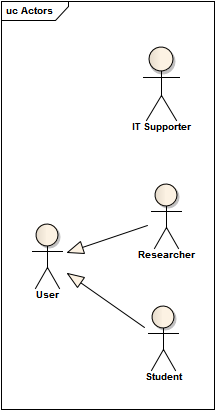
\includegraphics{../ea_files/generatedImages/Computational_platform/Actors.png}
		\caption{Actors of computational platform.}
		\label{app:cp:actors}
	\end{figure}
	\begin{figure}[!hbtp]
		\centering
		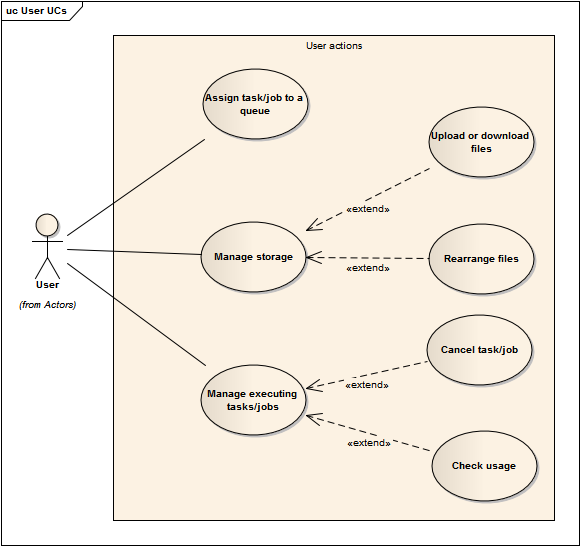
\includegraphics[width=\textwidth]{../ea_files/generatedImages/Computational_platform/UserUCs.png}
		\caption{User use cases in computational platform.}
		\label{app:cp:ucs}
	\end{figure}
	\begin{figure}[!hbtp]
		\centering
		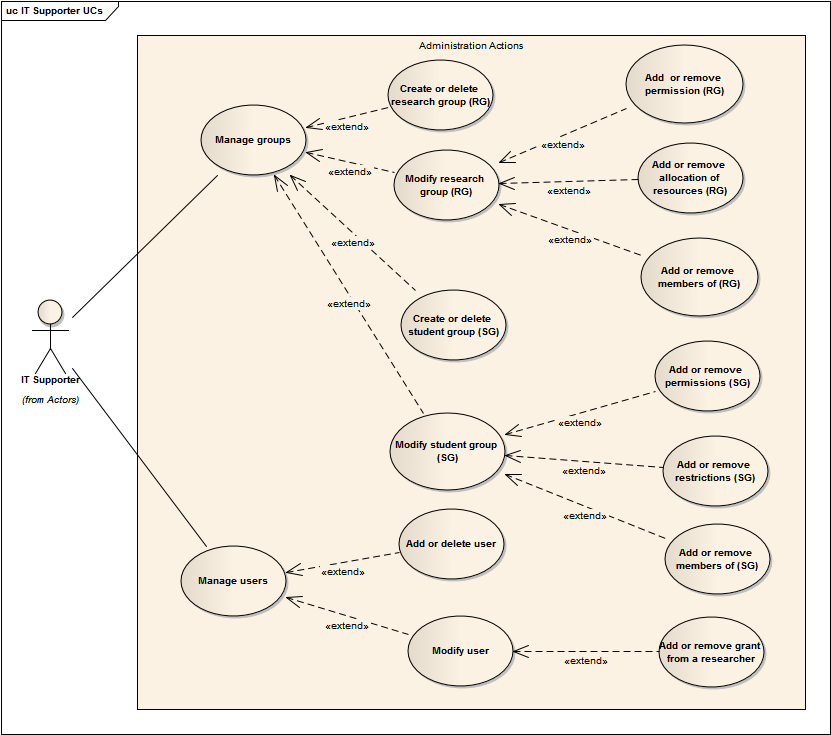
\includegraphics[width=\textwidth, angle=0]{../ea_files/generatedImages/Computational_platform/ITSupporterUCs.png}
		\caption{It Supporter use cases in computational platform.}
		\label{app:cp:itucs}
	\end{figure}
	\begin{figure}[!hbtp]
		\centering
		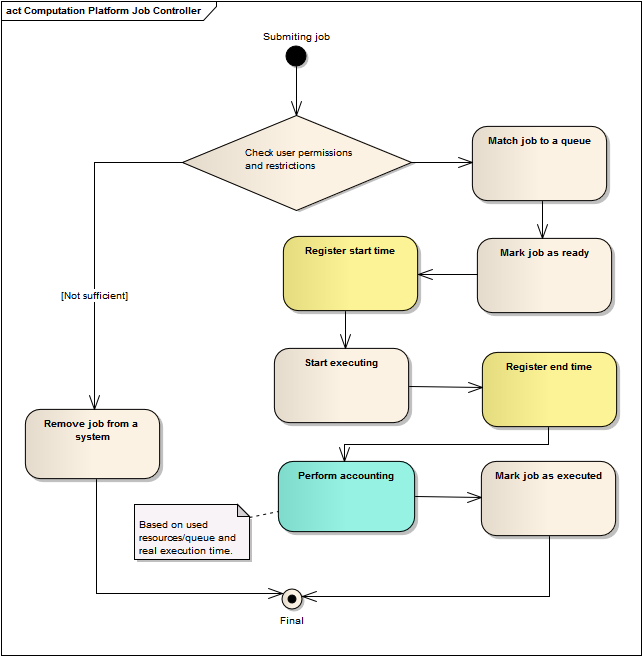
\includegraphics[width=\textwidth]{../ea_files/generatedImages/Computational_platform/ComputationPlatformJobController.png}
		\caption{Simplified computational platform job controller algorithm.}
		\label{app:cp:jobcontroller}
	\end{figure}
\clearpage
\subsection{Simulation Tool Diagrams}
	\begin{figure}[!hbtp]
		\centering
		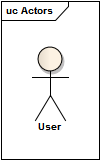
\includegraphics{../ea_files/generatedImages/Simulator/Actors.png}
		\caption{Actors of simulation tool.}
		\label{app:st:actors}
	\end{figure}
	\begin{figure}[!hbtp]
		\centering
		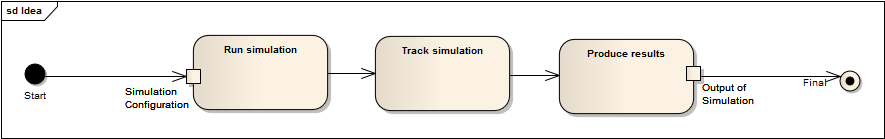
\includegraphics[width=\textwidth]{../ea_files/generatedImages/Simulator/Idea.png}
		\caption{Idea of simulation tool.}
		\label{app:st:idea}
	\end{figure}
	\begin{figure}[!hbtp]
		\centering
		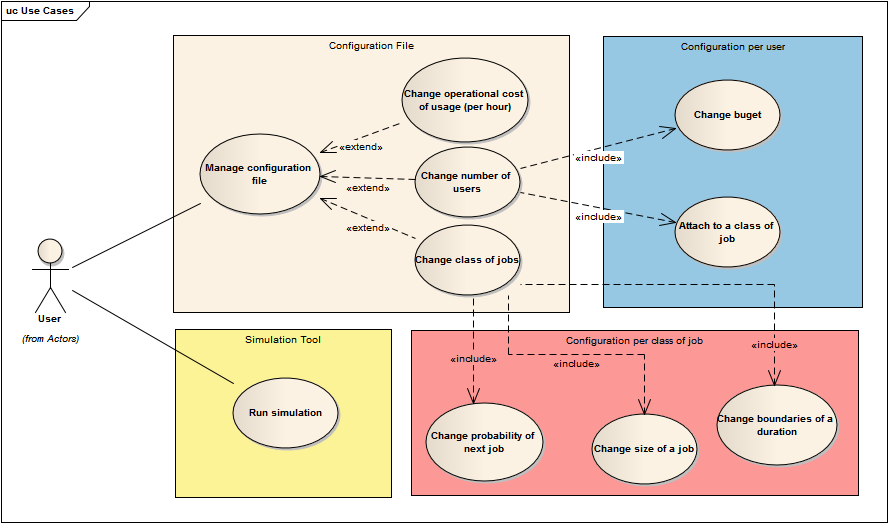
\includegraphics[width=\textwidth, angle=90, scale=1.4]{../ea_files/generatedImages/Simulator/UseCases.png}
		\caption{Use cases of simulation tool.}
		\label{app:st:ucs}
	\end{figure}
	\begin{figure}[!hbtp]
		\centering
		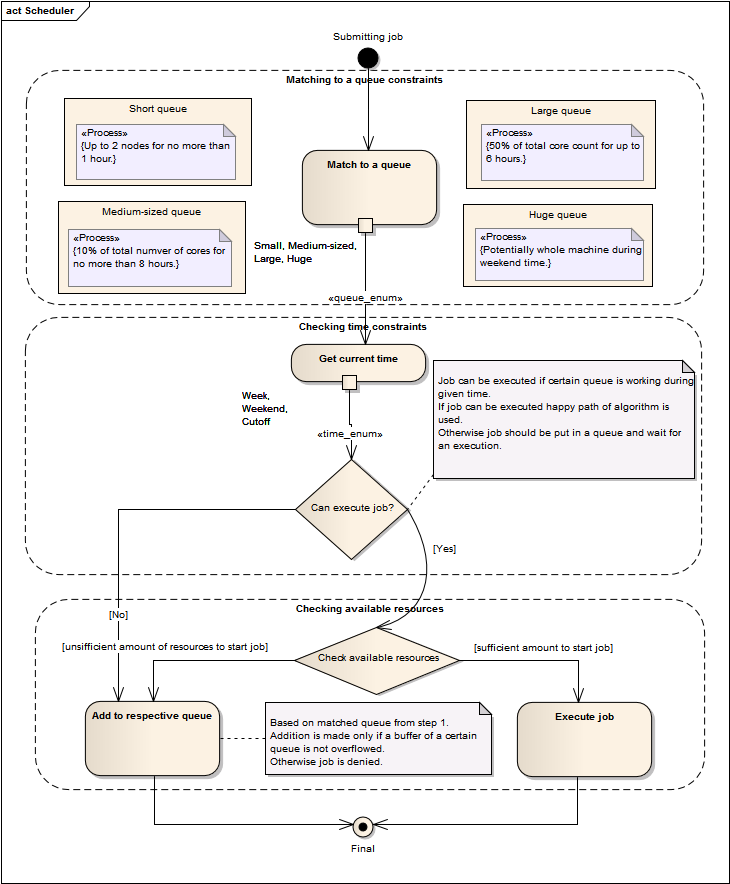
\includegraphics[width=\textwidth, angle=0, scale=1.0]{../ea_files/generatedImages/Simulator/Scheduler.png}
		\caption{Idea of scheduling algorithm in simulation tool.}
		\label{app:st:scheduer}
	\end{figure}
\section{Appendix C: To Be Determined List}
$<$Collect a numbered list of the TBD (to be determined) references that remain 
in the SRS so they can be tracked to closure.$>$

\end{document}
